\section{物体浮沉条件的应用}\label{sec:6-5}

浮沉条件在实际中有很多应用,下面简单介绍几个例子。

潜水艇是军事上的一种重要舰艇,它适于潜入水下航行,进行侦察或作战。
\CJKunderwave{潜水艇的潜水和上浮是靠改变自身重来实现的}。
在潜水艇的侧面有水舱(图 \ref{fig:6-9}),向水舱中充水时,潜水艇逐渐加重,潜水艇就逐渐潜入水中。
当水舱中充入适量的水时,潜水艇能够停留在水中任何深度处。
在潜水艇需要上浮时,就用压缩空气排出水舱中的水,使潜水艇变轻,从而浮出水面。

\begin{figure}[htbp]
    \centering
    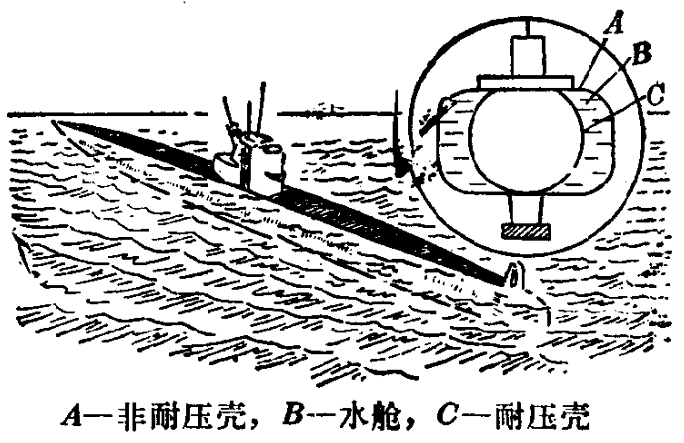
\includegraphics[width=0.6\textwidth]{../pic/czwl1-ch6-9}
    \caption{潜水艇}\label{fig:6-9}
\end{figure}

\begin{wrapfigure}[14]{r}{3.5cm}
    \centering
    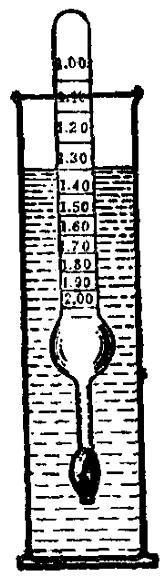
\includegraphics[width=2cm]{../pic/czwl1-ch6-10}
    \caption{比重计}\label{fig:6-10}
\end{wrapfigure}

由于潜水艇能够潜入水下,行动隐蔽,可以避免被敌人发现。
因此,在军事上用潜水艇侦察敌情,攻击敌舰。
在建设事业中,可以用潜水艇来进行海底考察,水下运输。

有一种测量液体密度的仪器,是利用物体浮在液面的条件工作的。
它是一根密封的玻璃管,管的下部装有小弹丸或水银,使它能够竖直地浮在液体中(图 \ref{fig:6-10})。
由于它受到的重力是一定的,它浮在液体中受到的浮力是一定的,
所以把它放在密度较大的液体中,它排开的液体较少,玻璃管浸入液面下的深度就小些;
把它放入密度较小的液体中,它排开的液体较多,玻璃管浸入液面下的深度就大些。
根据玻璃管浸入液体中的深度就可以测量液体的密度。
玻璃管上的刻度值有的标的是液体的密度与水的密度的比值,习惯上把具有这种刻度的仪器叫做\textbf{比重计}。
例如图 \ref{fig:6-10} 中比重计的读数是 1.3,就表示这种液体的密度是水的密度的 1.3 倍。

气体也有浮力,气球(图 \ref{fig:6-11})和飞艇(图 \ref{fig:6-12})就是利用空气的浮力升入高空的。
气球可以用来进行气象观测,如测定高空的风速、风向、温度、气压等,还可以用来研究高空大气的性质,进行通讯广播等。
飞艇可以用来进行空中运输,吊运货物等。


\begin{figure}[htbp]
    \centering
    \begin{minipage}{7cm}
    \centering
    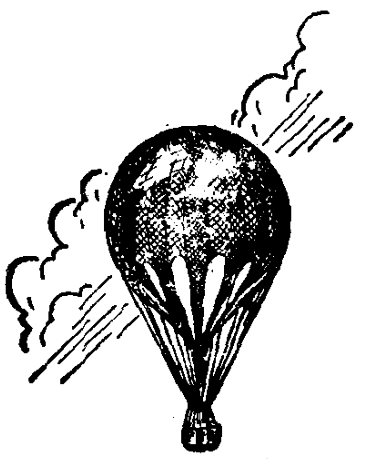
\includegraphics[width=4cm]{../pic/czwl1-ch6-11}
    \caption{气球}\label{fig:6-11}
    \end{minipage}
    \qquad
    \begin{minipage}{7cm}
    \centering
    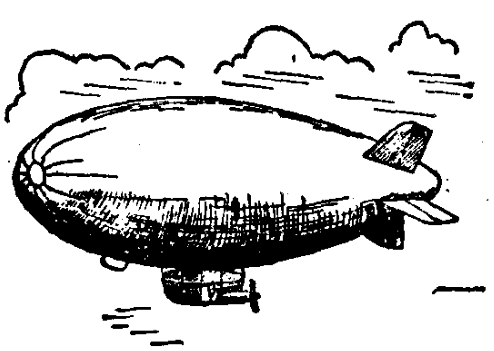
\includegraphics[width=5cm]{../pic/czwl1-ch6-12}
    \caption{飞艇}\label{fig:6-12}
    \end{minipage}
\end{figure}

气球和飞艇的主要组成部分是气囊,在气囊里面装着密度比空气小的气体,例如氢气\ 氦气或热空气。
气囊的下面挂着一个吊篮,可以装仪器、货物或乘人。
如果气球或飞艇本身加上所载的物体和人受到的重力小于气囊排开的空气重,也就是小于它们受到的浮力,气球或飞艇就能上升。
由于越到高空空气越稀薄,空气的密度越小,所以气球在上升的过程中受到的空气的浮力越来越小。
当升到一定高度,浮力等于重力时,它就不再上升,停留在这个高度上。
需要降落时,只要把气囊中的气体放出一部分,使气囊的体积减小,从而使受到的浮力减小,就可以使气球降回地面。
在飞艇上还装有发动机,可以驱使飞艇在空中飞行。



\lianxi

(1) 打捞沉船的时候,把一些盛着水的大金属箱沉入水里,拴在沉船上,然后用压缩空气把金属箱里的水压出来,
沉船就可以浮上来。这是什么道理?

(2) 我国汉代曾发明过一种做军事信号用的灯笼,它用很轻的竹篾扎成框架,用纸糊严,只在下面留口,
在灯笼的下面放一个小碟,盛上松脂。点燃松脂时,灯笼就能腾空而起,飞上高空(图 \ref{fig:6-13})。
这种灯笼升空的原理是什么?

\begin{figure}[htbp]
    \centering
    \begin{minipage}{7cm}
    \centering
    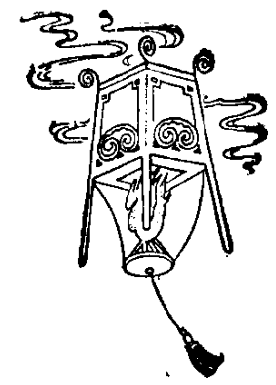
\includegraphics[width=4cm]{../pic/czwl1-ch6-13}
    \caption{}\label{fig:6-13}
    \end{minipage}
    \qquad
    \begin{minipage}{7cm}
    \centering
    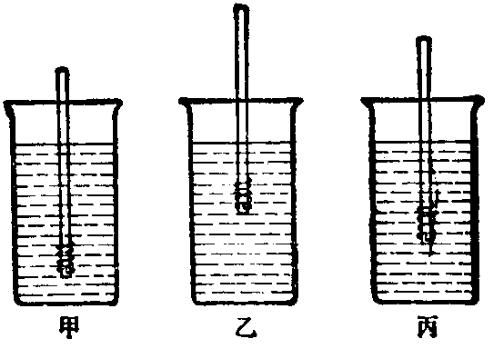
\includegraphics[width=6cm]{../pic/czwl1-ch6-14}
    \caption{}\label{fig:6-14}
    \end{minipage}
\end{figure}

(3) 传说三国时孙权送给曹操一只大象。大象很大,参观的人纷纷议论这只大象究竟有多重,
但是却想不出称大象的办法。这时曹操的儿子、年仅六岁的曹冲想出了一个办法。
他说只要把大象牵到船上去,看船沉下多少,在船舷上做个记号,然后把大象牵上岸。
再往船上装石头,使船沉到原来的记号处,称出这些石头有多重就知道大象多重了。
你能说出曹冲称象的道理吗?

(4) 在一根表面涂蜡的细木棍的一端绕着适量的铁丝,把它放到三种密度不同的液体里,
木棍浸入液体里的情况如图 \ref{fig:6-14} 所示。这三种液体的密度哪种最大?哪种最小?

(5) 有一方木块,把它放入水中时,露出水面的部分是它总体积的 $\dfrac{2}{5}$;
把木块放入另一种液体中时,它露出液面的部分减小为总体积的 $\dfrac{1}{3}$。
木块在这两种情况下受到的浮力是否相等?为什么?




